\section{Do Rewards Bias Exploration?}

\subsection{Modelling Exploration}
\begin{itemize}
    \item Rosenberg impements a markov chain model to for exploration behaviour. This model effectively memorizes turning statistics. 
    \item Across mice they observe four biases in node action decisions as follows:
    \item <insert description of biases>
    \item They implement a simplified 4-bias markov model and train these on each mouse to determine a weighting for each bias which reflects the mouses tendencies during exploration.
    \item We explore these models with respect to both
    \item a) the influence of maze and reward structure on exploratory behaviour,
    \item b) the generality of the different models
    \item The 4 biases are given as follows:
    \item 2 biases covering movement deeper into the maze: $P_{SF}$ is the probability that the mouse will move forward. $P_{SA}$ that it will alternate left and right actions at a T junction. 
    \item 2 biases covering movement out of the maze: $P_{BF}$ is the probability that the mouse will move forward through the junction. $P_{BS}$ that it will turn rather than go straight.
    \item The direct path from home to water port is achieved by the following sequence of actions: RLLRLR, where R is right and L is left
    \item While the direct path from water port to home is given by the sequence: STTTTTT, where S is straight, and T is turn
    \item We see that for the direct path to water, $P_{SF} = 1$ and $P_{SA} = 0.8$. Identically for the direct path home, $P_{BF} = 1$ and $P_{BS} = 0.8$.
    \item Thus drink and leave modes should have high values for these biases, and we observe this in <insert figure >
\end{itemize}

\begin{figure}
    \centering
    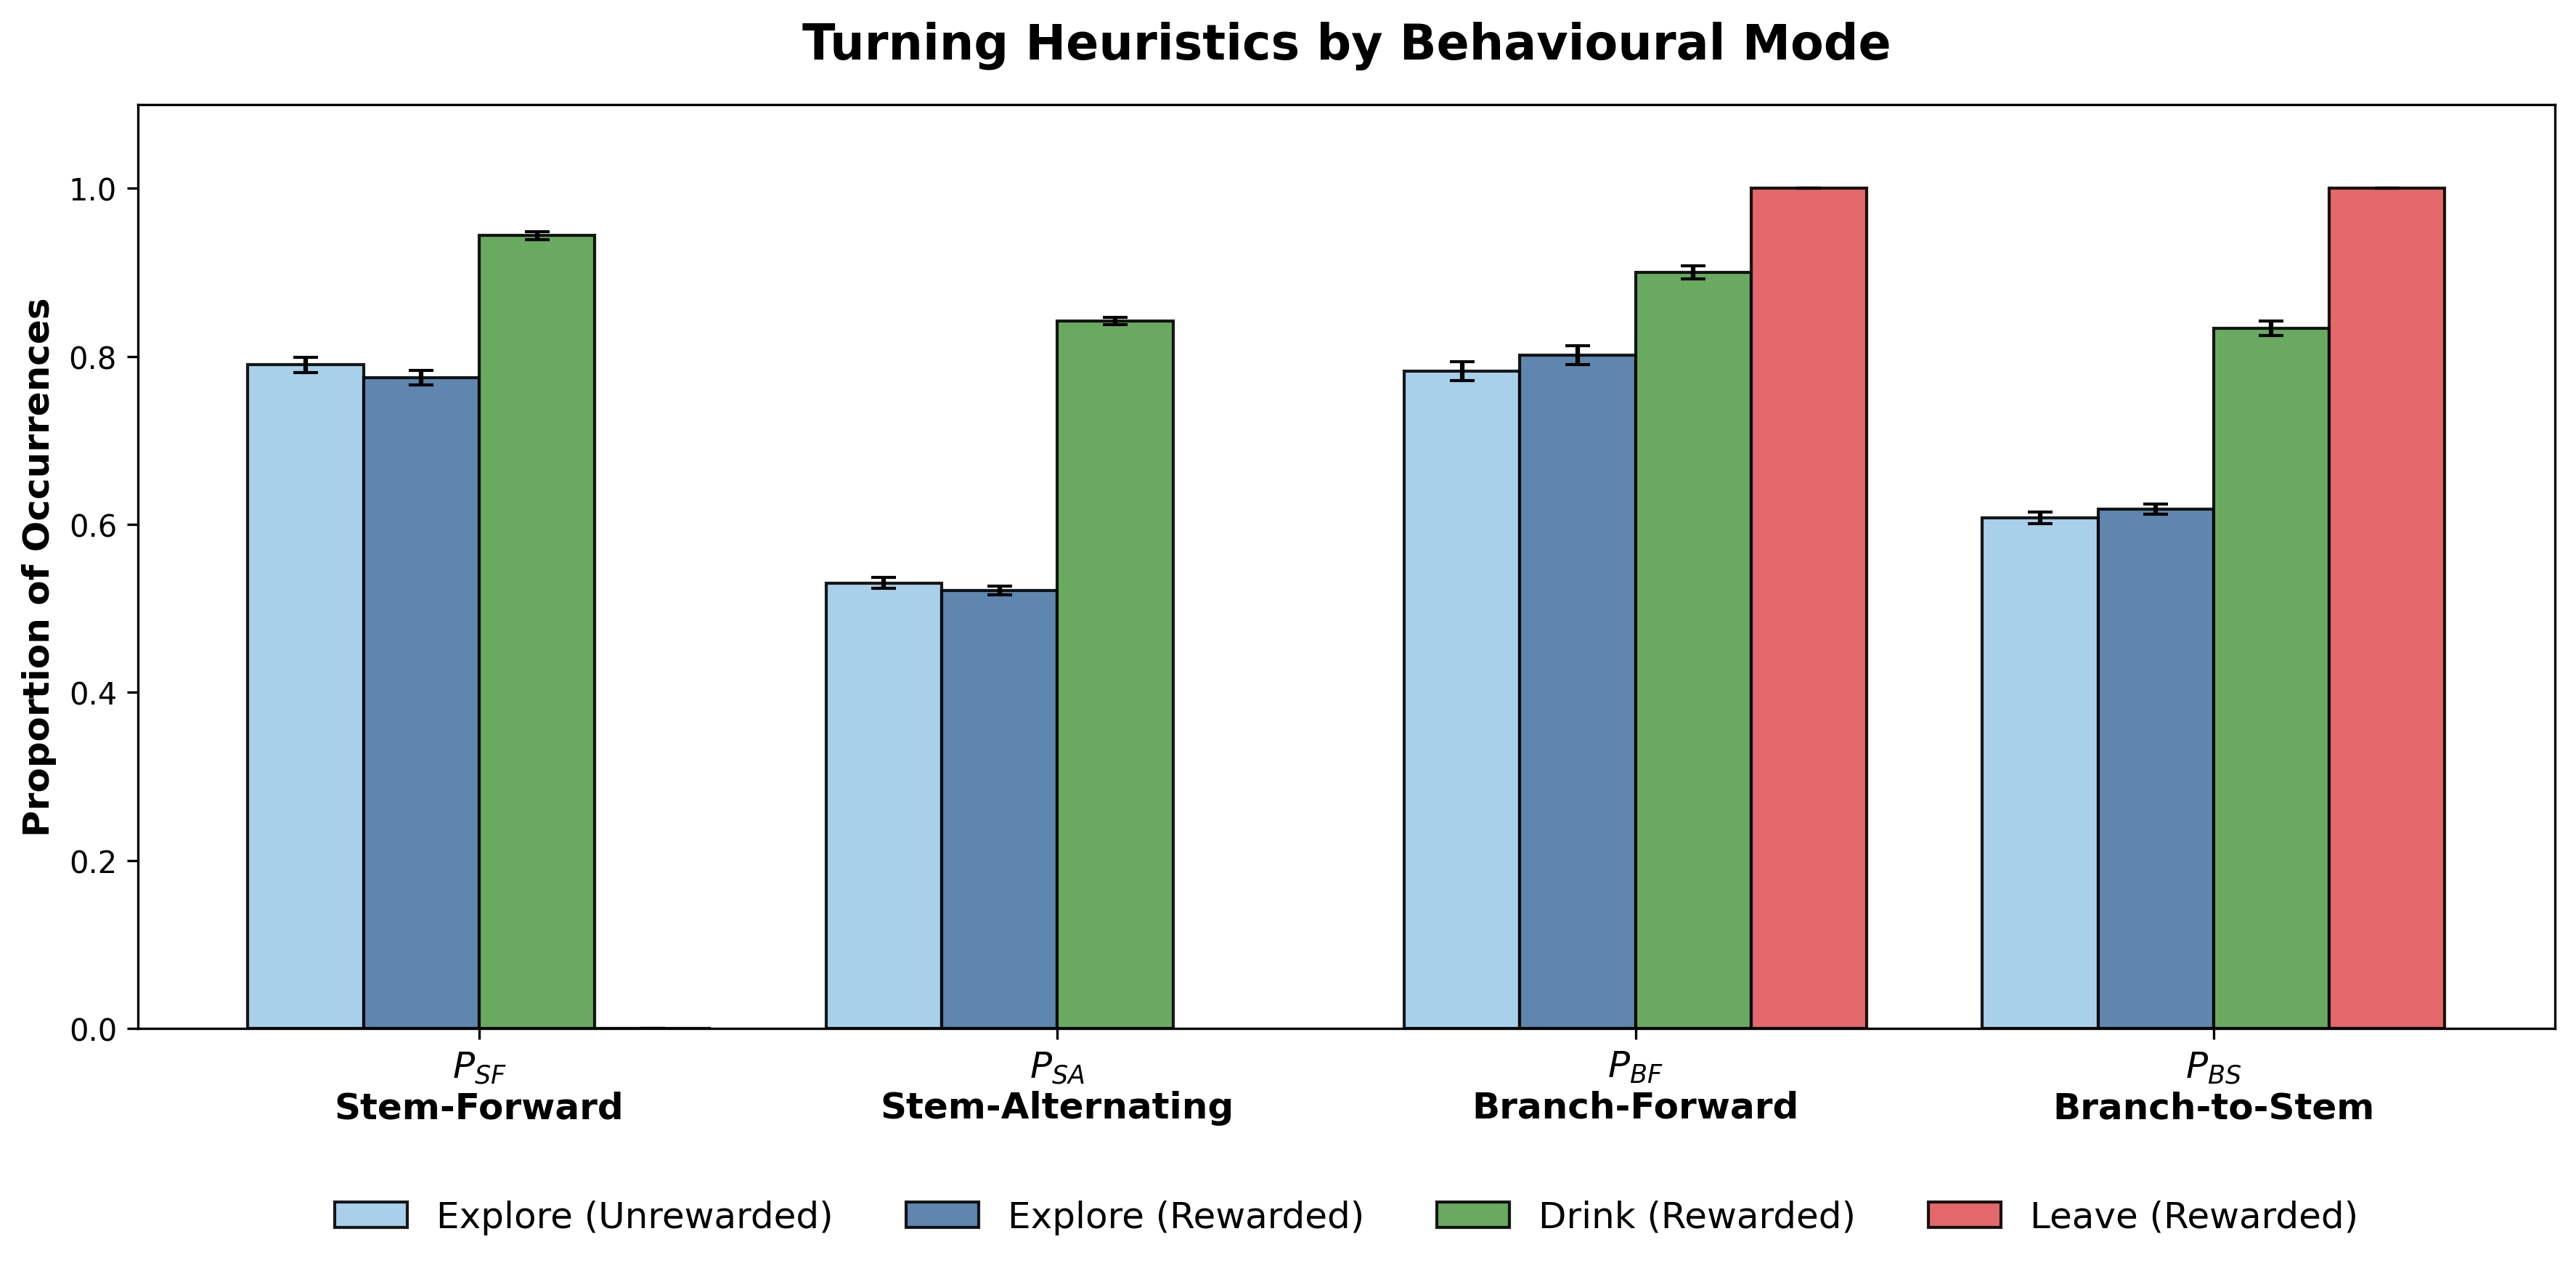
\includegraphics[width=\singlefigure]{figures/heuristics_by_behavioural_mode.png}
\end{figure}

\subsection{Do Models Generalise?}

\begin{itemize}
    \item We test the generalisaibility of the 4-bias models. We train one model per mouse on explore mode data for both rewarded and unrewarded groups. 
    \item We train them using a 5-fold cross validation, and test each model on each mouse by calculating the cross-entropy of model predictions against the 20\% test data and use a box plot to analyse the results.
    \item We make a number of observations. 
    \item For both groups, the cross-entropy has a range of 0.1, suggesting that there is a range of structured behaviour in exploration.
    \item The unrewarded mice tend to have a higher cross-entropy, suggesting that their exploration is more random.
    \item We also observe that models trained on the unrewarded mice generally perform better on the rewarded mice than on the target of training, again suggesting more randomness in exploration for unrewarded mice.
    \item Variance in cross-entropy of models trained on differnet mice from test have higher variance, though the range is small, suggesting that the 4 biases identified by Rosenberg represent generic eexploration rules which are consistent across mice.
\end{itemize}

\begin{figure}
    \centering
    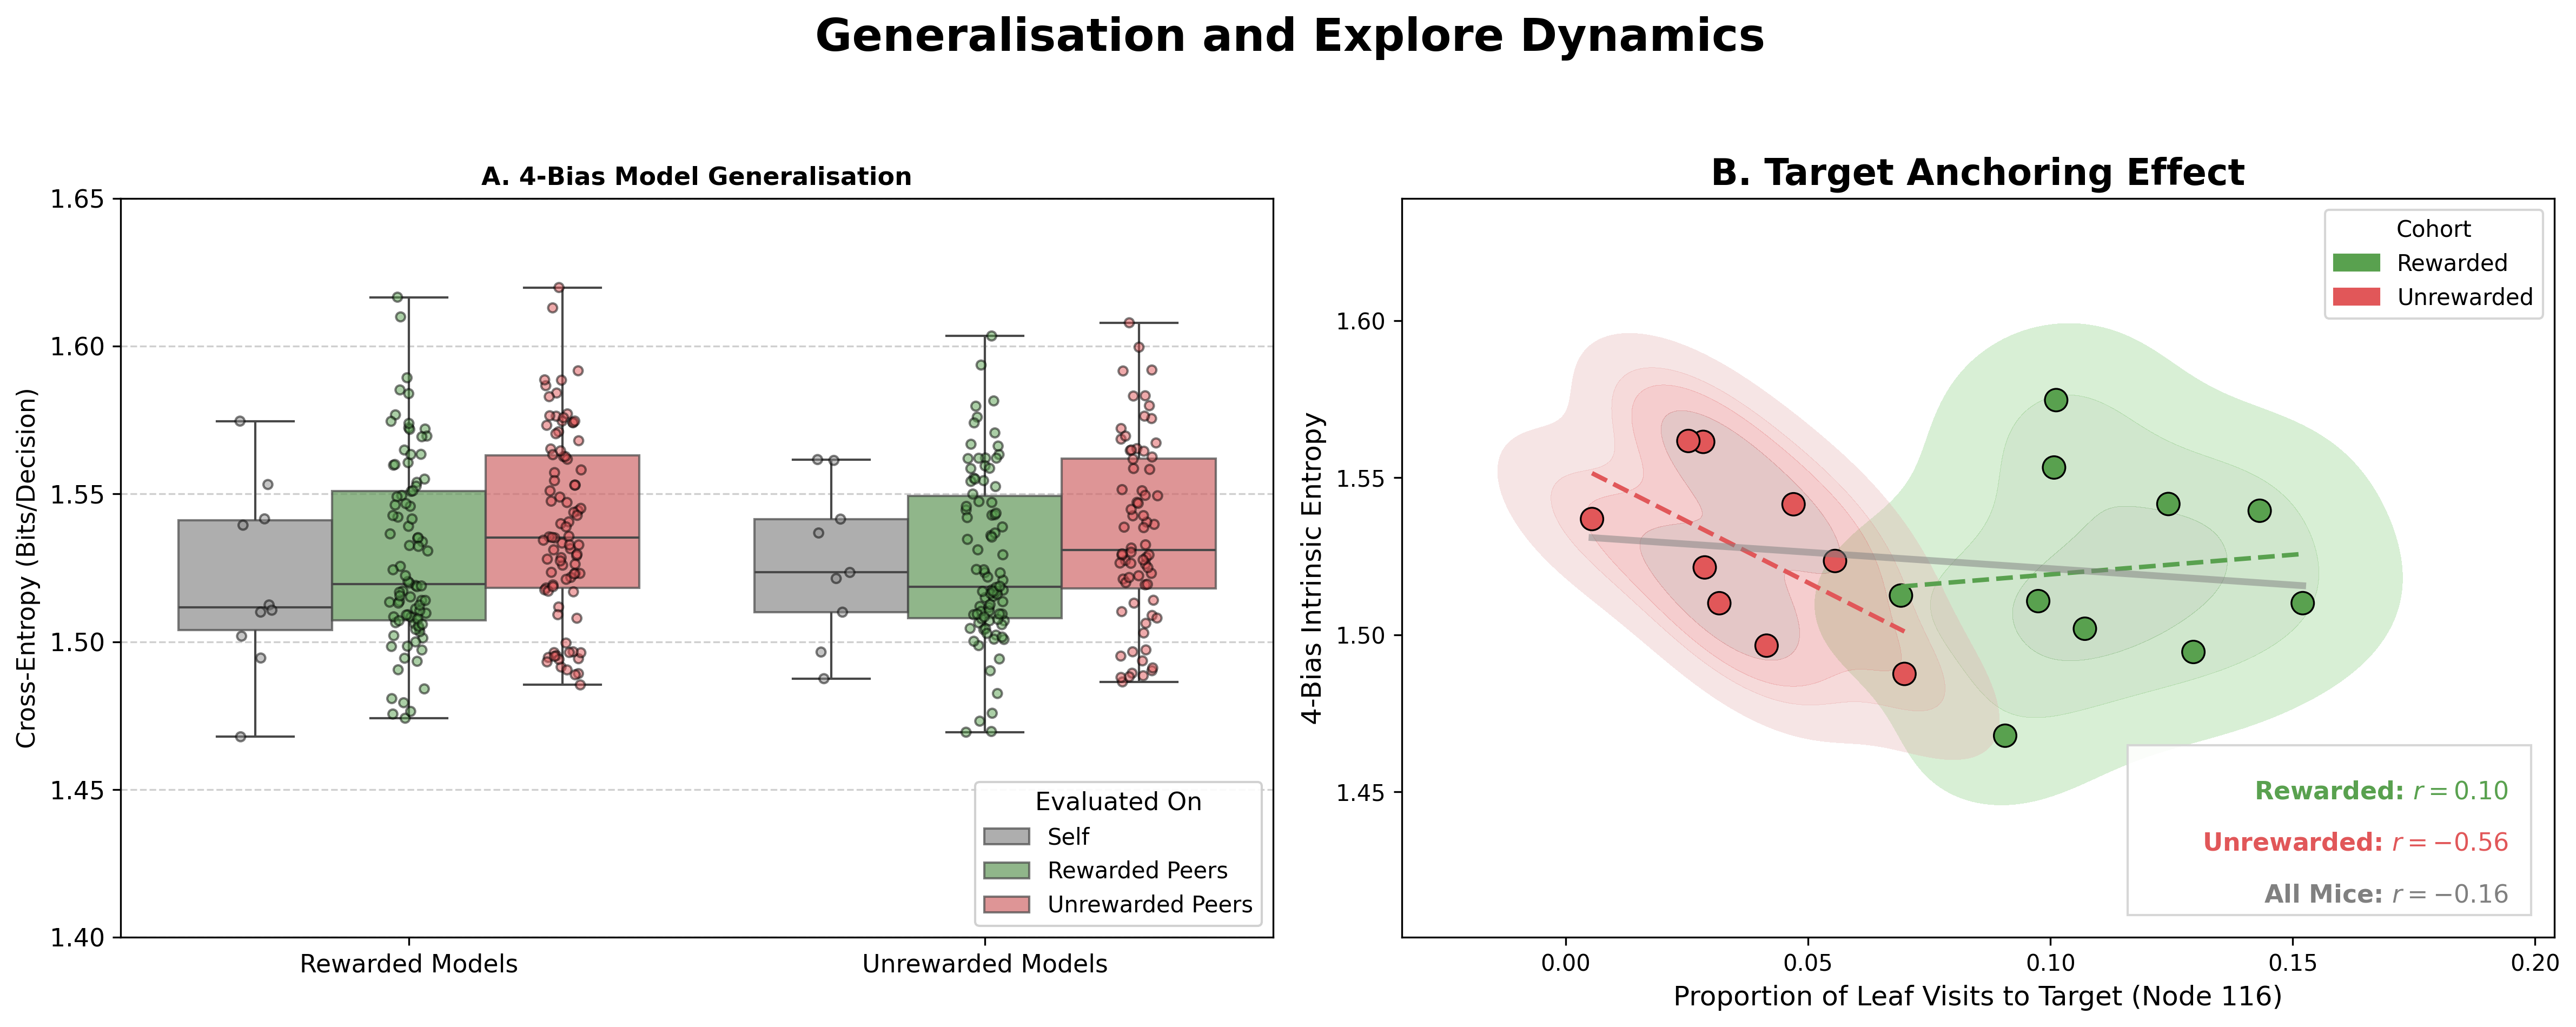
\includegraphics[width=\singlefigure]{figures/generalisation_and_anchoring_box.png}
\end{figure}

\subsection{Does the Water Port Still Matter?}

\begin{itemize}
    \item We revisit the question of whether the water port influences exploration.
    \item We plot the intrinsic entropy of mice (modelled and tested on 100\% of their data) against the proportion of leaf node visits made to the water port node (116).
    \item We note that since modelling is run on the explore mode data, the intrinsic exploration for the rewarded group actually excludes paths to the water port.
    \item As such, the bias should have been removed from modelling, and this is corroborated by the spherical distribution and near zero pearson correlation.
    \item However, visits to the water port have not been removed from the unrewarded mice since they are never in drink mode.
    \item We observe a correlation of -0.56 between the intrinsic exploration and the proportion of water port visits for the unrewarded mice.
    \item The more visits to the water port, the more structured their exploration.
    \item This may be indicative that the short paths, including paths to water port, discussed in <previous section>, and the tendency for mice to investigate node 116, may result in more structured exploration bouts.
    \item In future work, it may be useful to interrogate these more directed explorations, and possibly to classify an aditional behavioural mode which separates this behaviour.
\end{itemize}
